\documentclass{article}
\usepackage{graphicx}
\usepackage{caption,subcaption}
\usepackage{hyperref,float}
\usepackage[top=1.5in,bottom=1.5in,left=1.5in,right=1.5in]{geometry}
\usepackage{array,multirow}
\usepackage{multicol}

\setlength{\parindent}{0em}
\setlength{\parskip}{1em}

\title{CLI Usability}
\author{Tyler Cecil, Louis Jencka, Jesse Maes}

\begin{document}
\maketitle{}
\section{Background}
\label{sec:background}
In the lecture from the first day of HCI, we talked about the history of
computer user interfaces. The command line interface (CLI) was mentioned in a
slide, as an example of a historical type of interface. It was described as
“Efficient, precise, and fast.”

Unfortunately, this advanced interface has gained its power at the expense of
ease-of-use. Utilizing the CLI entails a “large overhead to learning set of
commands,” which is what has led to peculiar design goals for command line
interfaces. Commands and options are generally terse abbreviations, which are
very easy to memorize, but are not necessarily easy to learn.

As Computer Scientists, the CLI isn’t just relic of history; we make heavy use
it on a daily basis. It’s a powerful and highly flexible tool, useful for a
menagerie of tasks. For the beginner user, the shell can be an incomprehensible
nightmare - its blinking cursor against a blackened sky a stand-in for man’s
helpless struggle against death. Just as text editors have made leaps and bounds
in communicating essential contextual information, we believe the CLI can be
improved for beginning and advanced users alike.

%%% Local Variables:
%%% mode: latex
%%% TeX-master: "documentation"
%%% End:


\section{Problem Definition}
\label{sec:problem}
\begin{figure}[h]
  \centering
  \includegraphics[width=0.8\linewidth]{figures/sketch.png}
  \caption{A sketch of our problem design.}
  \label{fig:sketch}
\end{figure}

Shown above in \figure[fig:sketch] is the problem sketch for our project. The
frames are color-coded according to the model-view-controller (MVC) design
pattern: green is model; blue is view; red is controller.

The sketch begins
with a user, of any experience level, who interacts with the system via keyboard
and mouse. Their view into the system consists of a CLI window and a contextual
information window.

A user's input in passed from the interface through the
interaction engine. The interaction engine processes this text for command
suggestions, autocompletion, and automation. The OS's man pages, predefined
built-in patterns, the user's history, and the current state of the shell are
all used by the interaction engine for these features.

This system has a two-step state design, consisting of an 'active' state and a
'preview' state. For any command run, changes to the file system or to the state
of the shell are staged - saved in the preview state. If the user approves of
whatever changes were made, then the preview state is flushed to the active
state, and files on disk or environment variables are updated accordingly.


\section{Potential Users}
\label{sec:users}
\subsection{Beginners}
Our first imagined user is brand new to the shell, if not Linux itself. A
freshman CSE student, for example, would need to learn how to navigate a UNIX
operating system via its main interface - the shell. As a first-time Linux/BSD
user they would need to learn some basic information about how their system is
organized, and how to manipulate it. From their previous computer usage they
could be expected to understand the hierarchical nature of file systems, but
nothing more. What this user needs is to reach a baseline fluency in CLI usage:
how to navigate their file system; how to create and modify files; how to learn
more.
\begin{enumerate}
  \item No experience with UNIX operating systems
  \item No experience with a CLI
  \item No experience with the state inherent to a shell, mainly the current working directory
  \item No knowledge of what programming is, or how to automate tasks
  \item No knowledge of the anatomy of a command (command name, arguments, options, et cetera)
  \item No knowledge of the software available on their system
  \item No knowledge of basic OS tasks, such as installing software
  \item Has experience with common GUI techniques - click-to-open, drag-and-drop, et cetera
  \item Is uncertain
\end{enumerate}
\subsection{Casual Users}
Another potential user would be for scientists, engineers, or anyone with
experience as a technical computer user whose workflow could be more efficient
if they knew how to use the shell. The CLI can make it easier for users to
automate tasks and make precise changes to the files they are working on. These
users may already know how to complicated tasks on their computers, or even be
able to write programs. Many powerful tools insulate their users from the
details they would need to use the shell, such as Matlab, Maple, or Excel. An
information-rich user interface could help casual power users make the
transition to understand how to use their terminals for more complicated tasks
such as shell scripting and task automation.

\begin{enumerate}
  \item Understands the basics of how computers work and filesystems are organized
  \item Understands what computer programs are or has knowledge of how to program
  \item Is only familiar with a GUI, or is more comfortable with pointing and clicking than typing
  \item Regularly needs to perform some repetitive task on their computer, but does not imagine the task could be automated
  \item Finds themselves lost if/when they use the CLI - doesn’t understand the larger context of the system surrounding the shell
  \item Is unaware of most of the programs, commands, and command line options they could be using (has only seen the tip of the iceberg)
  \item Does not know how to apply technical knowledge or programming skills to system tasks in the CLI
\end{enumerate}
\subsection{Advanced User}
We also believe that advanced users who already know their way around the
command line could benefit from an information-rich shell. This user can be
expected to know by heart the commands they need to use, the details of how
their system is organized, and how to program in a shell language. Where the CLI
could stand improvement for these users is in providing more details on the
state of their system, and allowing a terser search of console-oriented
documentation.

\begin{enumerate}
  \item Deep understanding of OS structure and interfaces
  \item Mastery of command line usage
  \item Commonly constructs aliases and automates tasks
  \item Consults system documentation to find advanced command options
  \item Understands that task inference is frequently achievable from context in the shell
\end{enumerate}

%%% Local Variables:
%%% mode: latex
%%% TeX-master: t
%%% End:


\section{Tasks}
\label{sec:tasks}
\subsection{User Stories}
\emph{As a beginner, }
\begin{itemize}
  \item I want to compile my source code.
  \item I want to navigate to my source code.
  \item I want to be able to edit my source.
  \item I want easy access to information about what I am doing.
  \item I want to install the tools I need to make code.
  \item I want to know what I can do.
  \item I want to be able to open everything like I was able in windows.
  \item I want to know what my command is going to do.
  \item I want the same visual feedback a file browser gives me.
  \item I want to know how to utilize my shell’s history.
  \item I want to be able to easily and obviously perform common tasks.
  \item when I type a filename, I want the most common task associate with that file to be suggested.
  \item when I drag a file into the command line, I want that file name to be typed.
\end{itemize}

\emph{As a moderate user, }
\begin{itemize}
  \item I want to automate my workflow.
  \item I want the system to alert me when automation is an option.
\end{itemize}

\emph{As an expert user, }
\begin{itemize}
  \item I want tab-completion that is file-type aware
  \item I want heads up information about my system as I use it
\end{itemize}

\emph{As any user, }
\begin{itemize}
  \item I want to be able to copy and paste.
  \item I want to be able to drag a link into my shell and have the file be
    added to the current directory.
  \item I want the system to learn about my most common tasks.
  \item I want to know what options are available to me for a given command.
  \item I want contextual information displayed to me when composing commands.
  \item I want to view files in the current directory as I move through the
    system.
  \item I want to be able to undo what I've done.
\end{itemize}

\subsection{Hierarchical Analysis of Selected Tasks}
\begin{enumerate}
  \item As any user, I want to be able to undo what I've done.
  \begin{enumerate}
    \item Run a command
    \begin{enumerate}
      \item Know what command to run
      \item Write the command
    \end{enumerate}
    \begin{enumerate}
      \item Understand the results of the command
      \begin{enumerate}
        \item View what files/directories/settings were changed
        \item View how they were changed
      \end{enumerate}
    \end{enumerate}
    \item Undo a command
  \end{enumerate}

  \item As a beginner, I want to know what I can do with a file.
  \begin{enumerate}
    \item Specify a file
    \begin{enumerate}
      \item See what files are in my current working directory
      \item Select one of those files
    \end{enumerate}
    \item View the available commands
    \begin{enumerate}
      \item View a list of what commands would be useful for that file
      \item View what each command does
    \end{enumerate}
    \item Run a command on the file
    \begin{enumerate}
      \item Select a command
    \end{enumerate}
  \end{enumerate}

  \item As a casual user, I want to automate my workflow.
  \begin{enumerate}
    \item Specify a task which needs to be run many times
    \item View suggestions on how to run that task
    \item Select an automation technique
  \end{enumerate}

  \item As a beginner, I want to know what the command is going to do.
  \begin{enumerate}
    \item Specify a command
    \item View that command’s effects
    \begin{enumerate}
      \item View which files are going to be affected
      \item View how those files are going to be affected
    \end{enumerate}
    \item Chose whether to run the command or not
  \end{enumerate}

  \item As an expert user, I want heads-up information about my system as I use it.
  \begin{enumerate}
    \item See what the state of my session is
    \begin{enumerate}
      \item View background jobs
      \item View possible commands based on the current context
      \begin{enumerate}
        \item Take local files into account
      \end{enumerate}
      \item View the ways the current session has been altered - non-normal
      environment variables, virtual environments, et cetera.
    \end{enumerate}
  \end{enumerate}
\end{enumerate}
%%% Local Variables:
%%% mode: latex
%%% TeX-master: t
%%% End:


\section{Existing Systems}
\label{sec:existing}
While there exists no application that cover all of the contextual and adaptive
features discussed in this paper, the following existing systems tackle many of
our ideas for a richer shell.

\subsection{xterm}
While there exists no application that covers all of the contextual and adaptive
features discussed in this paper, the following existing systems tackle many of
our ideas for a richer shell.
\begin{figure}[h]
  \centering
  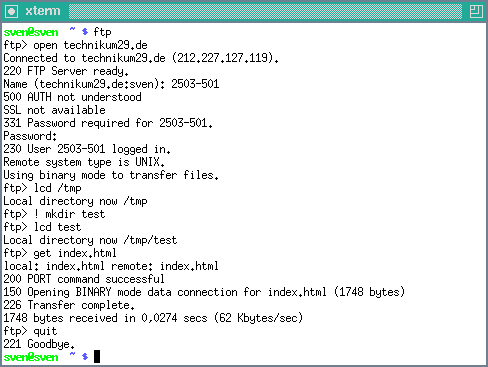
\includegraphics[width=0.8\linewidth]{figures/existing/xterm.png}
  \caption{An xterm window.}
  \label{fig:xterm}
\end{figure}

\subsection{iterm2}
iterm2, like xterm, essentially just provides a terminal emulator, which in turn
provides a shell. However, it is able to provide far more contextual information
than that of xterm. The shell can alert the terminal emulator itself about the
state of the system (such as current git status), as well as embed images into
the text result.
\begin{figure}[h]
  \centering
  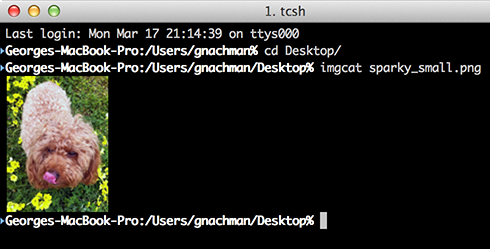
\includegraphics[width=0.8\linewidth]{figures/existing/iterm2.png}
  \caption{An iTerm 2 window, with inline images.}
  \label{fig:iterm}
\end{figure}

\subsection{zsh / Fish}
Both zsh and fish are shell programs designed to be more usable alternatives to
bash. A large part of this usability revolves around autocompletion and
suggestion. Fish will suggest command as you type (though it is not
bash-compatible). Zsh allows arbitrary autocompletion to be added to the system.
\begin{figure}[h]
  \centering
  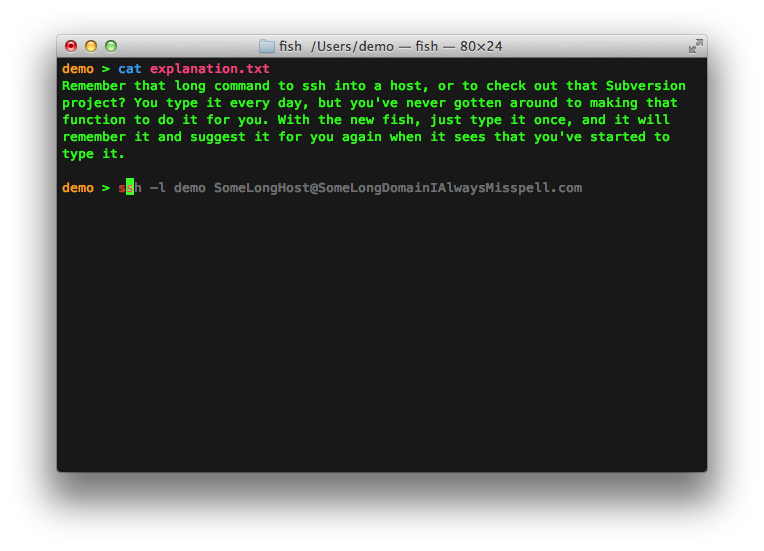
\includegraphics[width=0.8\linewidth]{figures/existing/fish.png}
  \caption{A fish shell, showing a suggested input.}
  \label{fig:iterm}
\end{figure}

\subsection{Explain Shell}
Explain shell is an educational tool which will break up a command, and explain
how it worked and what it means. This tool does not itself provide a shell, but
it does provide a tool which can be used to learn and understand bash and
related programs.
\begin{figure}[h]
  \centering
  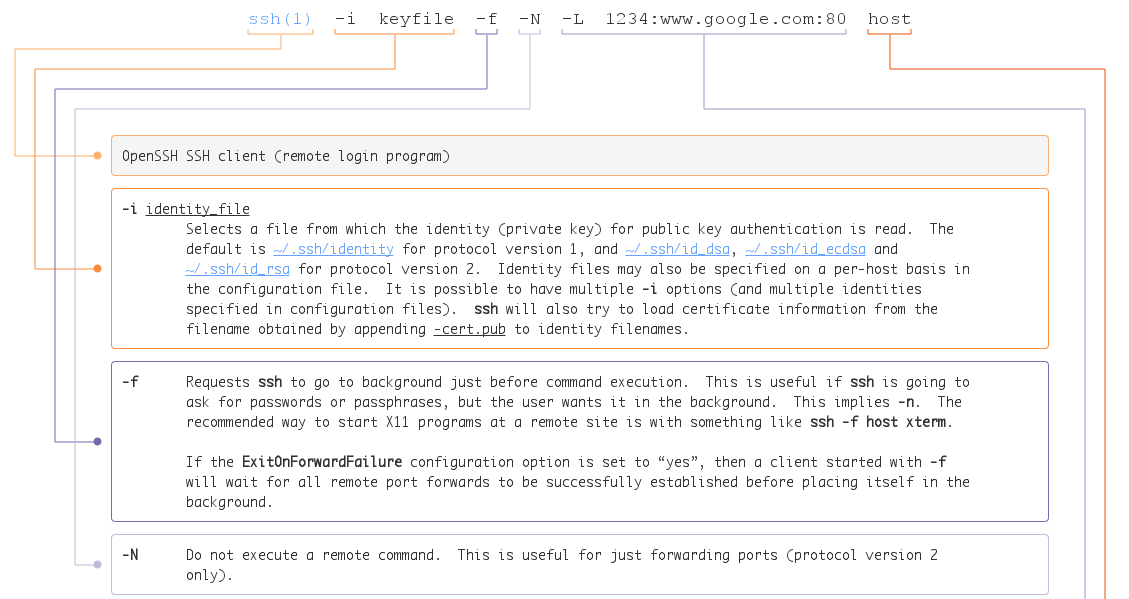
\includegraphics[width=0.8\linewidth]{figures/existing/eplainshell.png}
  \caption{A screen shot of explain shell breaking down a command.}
  \label{fig:iterm}
\end{figure}

\subsection{Jupyter}
Project jupyter is a modular, web based shell, designed for use with data
analytic languages (such as Julia, Python, and R). It allows graphical response
to commands, and let’s users distribute entire “sessions” of use. An important
feature is once a command is run, the user can edit the command. This chance
will then propagate through the history.
\begin{figure}[h]
  \centering
  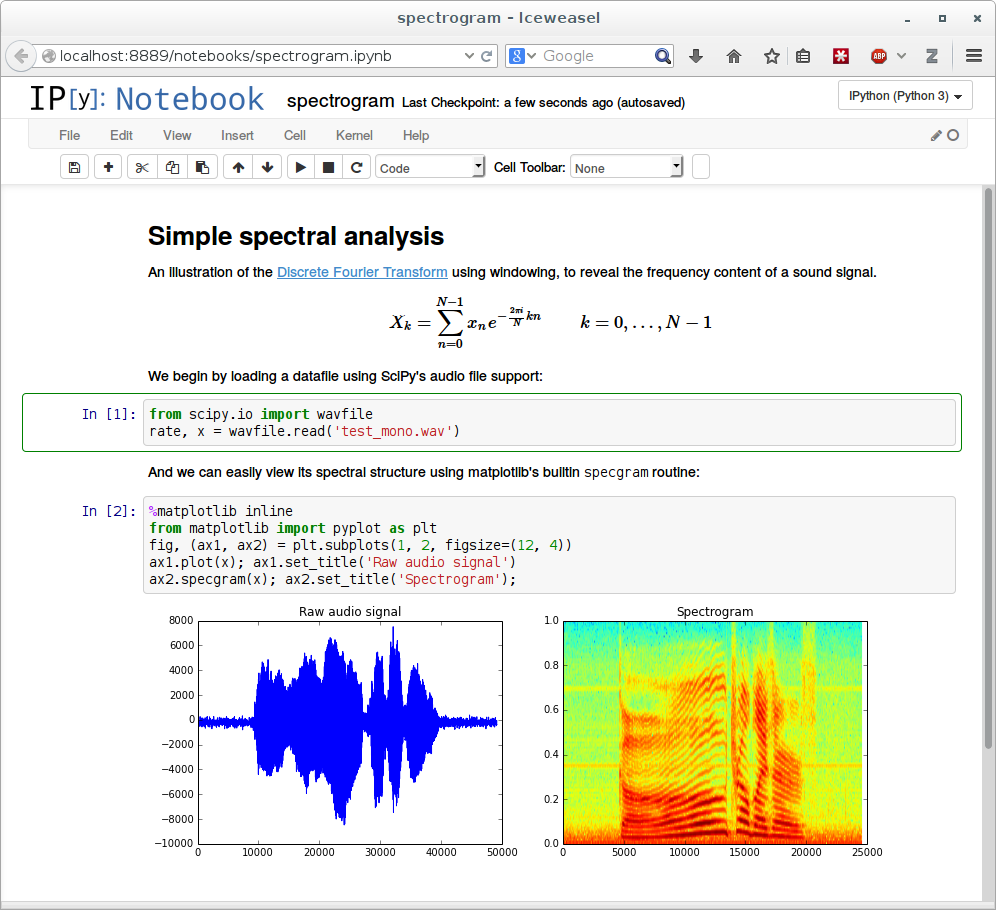
\includegraphics[width=0.8\linewidth]{figures/existing/ipython.png}
  \caption{An interactive jupyter session.}
  \label{fig:iterm}
\end{figure}

\subsection{Comparison of Features}

\begin{table}[h]
  \centering
  \begin{tabular}{|l|r|r|r|r|r|r|}
    \hline
    & This & \texttt{xterm} & iTerm 2 & \texttt{zsh}/\texttt{fish}
    & Explain Shell & Jupyter \\\hline
    Undo & V & X & X & X & X & V \\\hline
    File Actions & V & X & X & O & X & O\\\hline
    Automation Assistance & X & X & X & X & X & X\\\hline
    Command Results & V & X & X & X & V & O\\\hline
    Heads-Up Information & V & O & V & V & X & V\\\hline
  \end{tabular}
  \caption{Comparision of features. V -- able to perform the task, X -- unable
    to perform the task, O -- able to perform the task with poor interactive
    design.}
  \label{tab:features}
\end{table}
%%% Local Variables:
%%% mode: latex
%%% TeX-master: t
%%% End:



\section{Task Navigation (Design Alternatives)}
\label{sec:tas_nav}
For each of the main tasks provided in Section \ref{sec:tasks}, we analyze the
ways in which these tasks could be actualized. Each actualization is represented
with three separate diagrams showing the flow of actions.

\subsection{Undoing Actions}

In this task, the user needs to be able to be able to revert an action they have
just performed (something that is particularly useful for beginners to the
command line environment).
\begin{figure}[H]
  \centering
  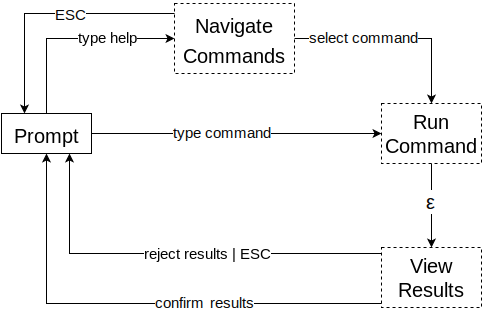
\includegraphics[width=0.8\linewidth]{figures/alternatives/undo_a.png}
  \caption{A breakdown of the procedure for undoing actions.}
  \label{fig:undoa}
\end{figure}

Figure \ref{fig:undoa} demonstrates a method which allows the user to see the
results of their actions, and then chose whether or not to carry it out.

\begin{figure}[H]
  \centering
  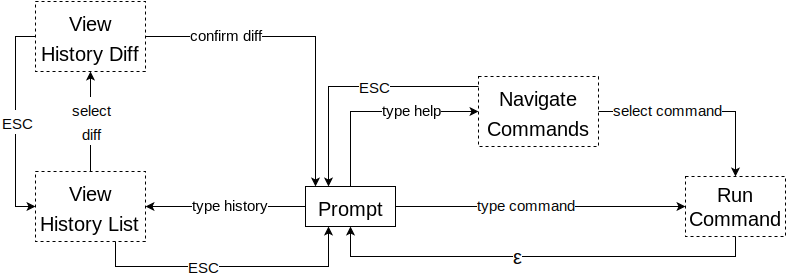
\includegraphics[width=0.8\linewidth]{figures/alternatives/undo_b.png}
  \caption{A breakdown of the procedure for undoing actions.}
  \label{fig:undob}
\end{figure}

A scheme that gives perhaps more undo ability (yet less pedagogical value) is
the ability to brows the history of your commands and the states they
represented. Figure \ref{fig:undob} shows such a scheme.

\begin{figure}[H]
  \centering
  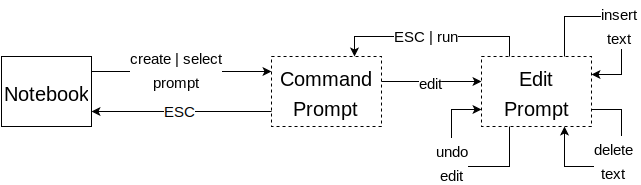
\includegraphics[width=0.8\linewidth]{figures/alternatives/undo_c.png}
  \caption{A breakdown of the procedure for undoing actions.}
  \label{fig:undoc}
\end{figure}

Another common way to deal with this problem is the style that is used by the
\emph{iPython} notebook \--- displaying the whole command history, and allowing
the user to change the text of the commands that were previously entered. Figure
\ref{fig:undoc} shows such a scheme.

\subsection{Discovery}

Users commonly want to know what they can do with given file types. We want to
provide the user with the knowledge of how to continue with their files.

\begin{figure}[H]
  \centering
  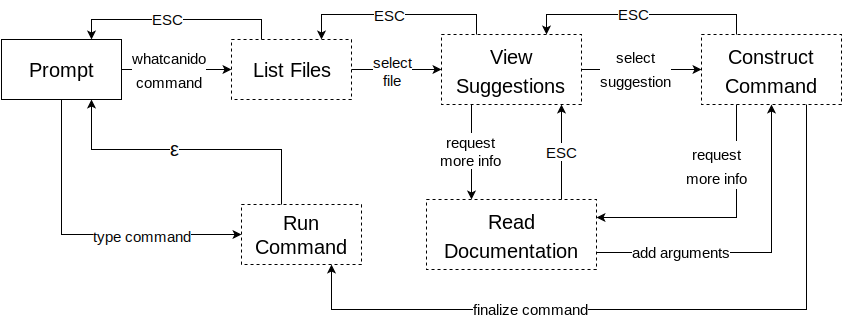
\includegraphics[width=0.8\linewidth]{figures/alternatives/file_a.png}
  \caption{A breakdown of the procedure for undoing actions.}
  \label{fig:disca}
\end{figure}

In Figure \ref{fig:disca} we present a model where first a file is selected. Once
the selection has been made, the shell can provide a list of ``what to do next''
options. This represents a more reverse polish style of shell navigation.

\begin{figure}[H]
  \centering
  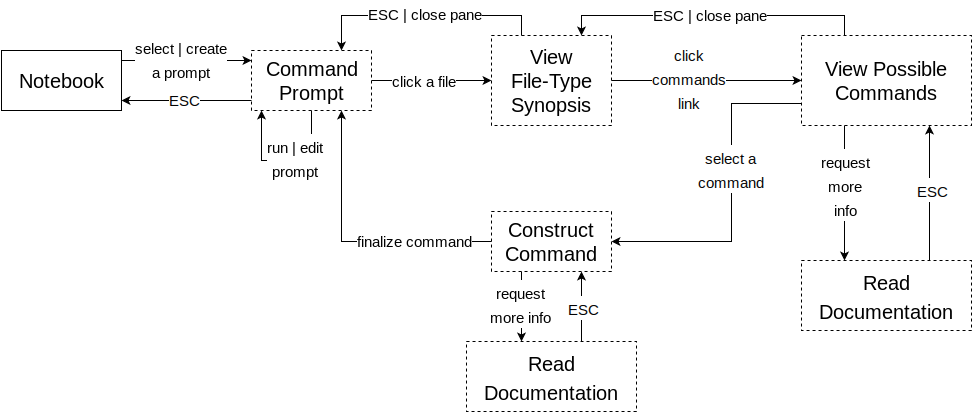
\includegraphics[width=\linewidth]{figures/alternatives/file_b.png}
  \caption{A breakdown of the procedure for undoing actions.}
  \label{fig:discb}
\end{figure}

An alternative to this, again, would be a notebook style interface, with a mouse
oriented approach. In this, we can select files, and can optionally be presented
with a list of actions.

\begin{figure}[H]
  \centering
  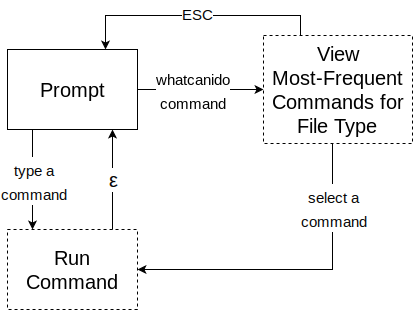
\includegraphics[width=0.8\linewidth]{figures/alternatives/file_c.png}
  \caption{A breakdown of the procedure for undoing actions.}
  \label{fig:discc}
\end{figure}

Figure \ref{fig:discc} shows the simplest way to implement this feature \--- a
special command to ask ``what is the most common task to perform on this file
type.''

\subsection{Workflow Automation}

Commonly users are performing repetitive tasks on a related set of files. They
may not understand that their workflow could be automated, or how to automate
things. The onus would then be on our software to detect common situations as
well as repetitive situations, and alert and assist the user in streamlining
their work.

\begin{figure}[H]
  \centering
  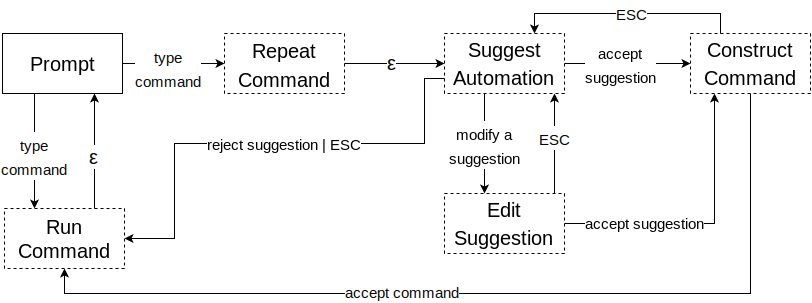
\includegraphics[width=0.8\linewidth]{figures/alternatives/automate_a.png}
  \caption{A breakdown of the procedure for undoing actions.}
  \label{fig:autoa}
\end{figure}

In Figure \ref{fig:autoa} we show perhaps the most obvious way to perform this
sort of automation \--- detect repeated commands, and suggest an automation path
(such as building a for loop). This will serve as a good, non-invasive method,
that will alert the user of features of the shell.

\begin{figure}[H]
  \centering
  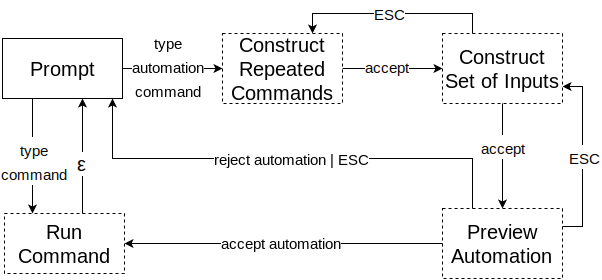
\includegraphics[width=0.8\linewidth]{figures/alternatives/automate_b.png}
  \caption{A breakdown of the procedure for undoing actions.}
  \label{fig:autob}
\end{figure}

The user, however, could be provided with an ``automate'' command, prompting
this system to provide automation suggestions. This would be an easier path to
pursue, but leave more responsibility for the user. Figure \ref{fig:autob} shows
such a scheme.

\begin{figure}[H]
  \centering
  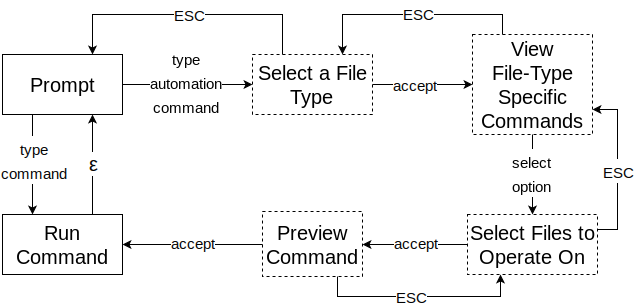
\includegraphics[width=0.8\linewidth]{figures/alternatives/automate_c.png}
  \caption{A breakdown of the procedure for undoing actions.}
  \label{fig:autoc}
\end{figure}

Finally, we could boil all automation commands down to batch processes on
related files. Figure \ref{fig:autoc} shows how the user may select related files,
and then build up a command to operate on all files.

\subsection{Preview Command}

Commonly users are not sure how what the results of their commands will be. We
feel being provided with a ``preview'' of commands may help build confidence in
the shell.

\begin{figure}[H]
  \centering
  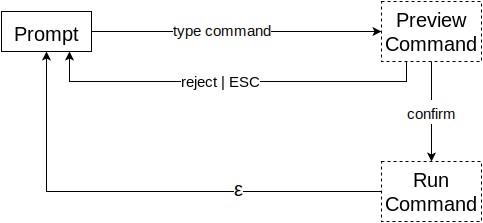
\includegraphics[width=0.8\linewidth]{figures/alternatives/preview_a.png}
  \caption{A breakdown of the procedure for undoing actions.}
  \label{fig:preva}
\end{figure}

An easy way to achieve this would be to preview the command while it is being
constructed, perhaps in the context window we have described. The user can then
fluidly work in the shell, seeing results before they occur.

\begin{figure}[H]
  \centering
  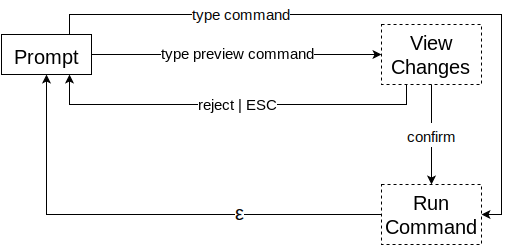
\includegraphics[width=0.8\linewidth]{figures/alternatives/preview_b.png}
  \caption{A breakdown of the procedure for undoing actions.}
  \label{fig:prevb}
\end{figure}

Figure \ref{fig:prevb} however would remove this as being the default behavior,
and allow the users to request a preview. The rest of the workflow would remain
unchanged.

\begin{figure}[H]
  \centering
  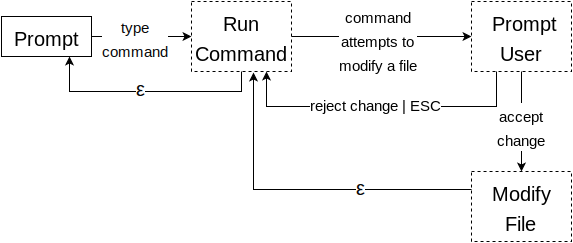
\includegraphics[width=0.8\linewidth]{figures/alternatives/preview_c.png}
  \caption{A breakdown of the procedure for undoing actions.}
  \label{fig:prevc}
\end{figure}

Finally, Figure \ref{fig:prevc} shows a case when previews are only used when
the shell detects a chance will be made to any files (probably the time when
users are most uncomfortable). This way the users are not constantly burdened
with previews, and only shown then when they really matter.

%%% Local Variables:
%%% mode: latex
%%% TeX-master: t
%%% End:


\section{Possible Interaction Techniques}
\label{sec:interact}
As this is an addition to the CLI, and not a departure from it, we intend to
keep the keyboard as the main focus. All new interfaces should be navigable by
keyboard, if not least primarily so. For users new to a CLI, however, they can
be assumed to be most comfortable with interacting via a mouse. We imagine that
for the novice and casual user alike, a hybrid interface could be highly useful.

The Gestalt Principles

Proximity --- In the shell there is a fixed amount of space between lines and
individual characters is fixed. However, textual output can still take advantage
of the principle of proximity by using whitespace to separate items that should
not be grouped together. This achieves the goal of grouping related objects in a
text-based interface.

Similarity --- Text mainly conveys semantic information, and we can use a few
techniques to visually tag that information so that the user can easily
determine the “type” of the text they’re reading and writing. Specifically,
automatically making use of output coloring and syntax highlighting can help CLI
a user pick apart information and group similar words within the buffer.

Past Experience --- Most importantly, we need to appeal to the experiences of both
novice and advanced users. Those who have never used the shell will expect their
filesystem to be presented to them in a way that reminds them of a file browser
- which is why we want to include a graphical pane which can be used to fill in
commands equivalent to point and click actions. More advanced users will be more
familiar with the basics of common commands, and can benefit from command
completion that will make it easier to type the things that they type most
often.

Color and light patterns could be used to convey information about the current
session. In class the structure of eyes was discussed, with a focus on what sort
of light is most easily noticed by different sections of they eye. In a
text-based interface this theory could be used to craft notifications that catch
the user’s attention based on the distance of the notification from the user’s
likely focus on the screen.

%%% Local Variables:
%%% mode: latex
%%% TeX-master: t
%%% End:


\section{Interface Design}
\label{sec:interface}
\subsection{Command Info}

\begin{figure}[H]
  \centering
  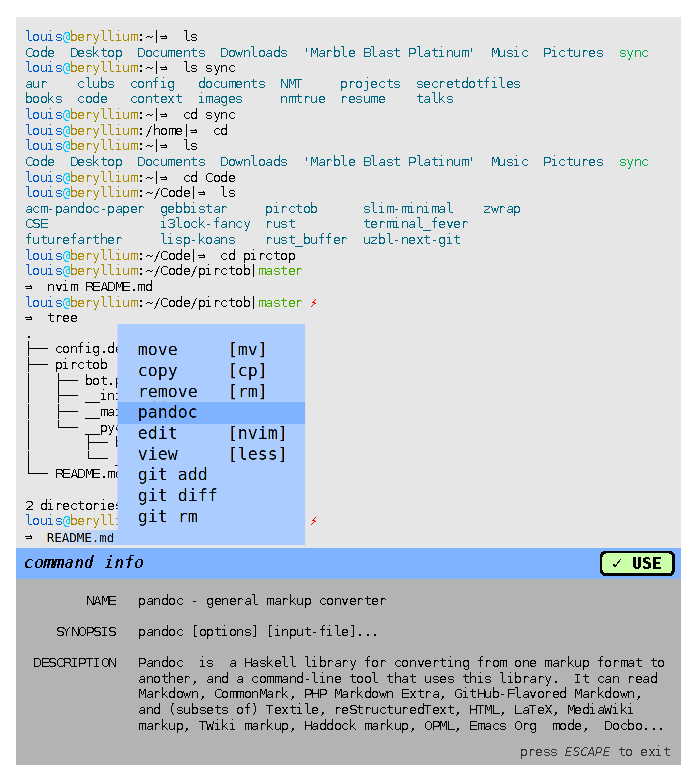
\includegraphics[width=0.8\linewidth]{figures/interface/files.eps}
  \caption{A mockup of the autocomplete dialog with the command info window}
  \label{fig:cmdinfo}
\end{figure}

Figure \ref{fig:cmdinfo} illustrates our idea for the autocomplete dialog. The
user can access the dialog by tab-completing the command they are typing, or
clicking on a the name of a file in the output of any command. The dialog box
can show a list of possible commands, determining which suggestions are most
likely based on command history, the current working context, or the type of the
file to be acted on. The autocomplete open remains open, leaving the user a
trail of ``breadcrumbs'' which can lead them back to other commands' information
windows.

The command info window is parsed from the man pages of the suggested commands,
and the layout is right/left aligned to make it easier to read. The window is
mainly a menu page for the particular command the user is interested in, but
doubles as an input form for the CLI. The possible command line options that
will appear in the documentation can be treated as form controls, (conceptually
similar to checkboxes), which allow the user to interactively build commands by
clicking or tabbing through.

\subsection{Undo Window}

\begin{figure}[H]
  \centering
  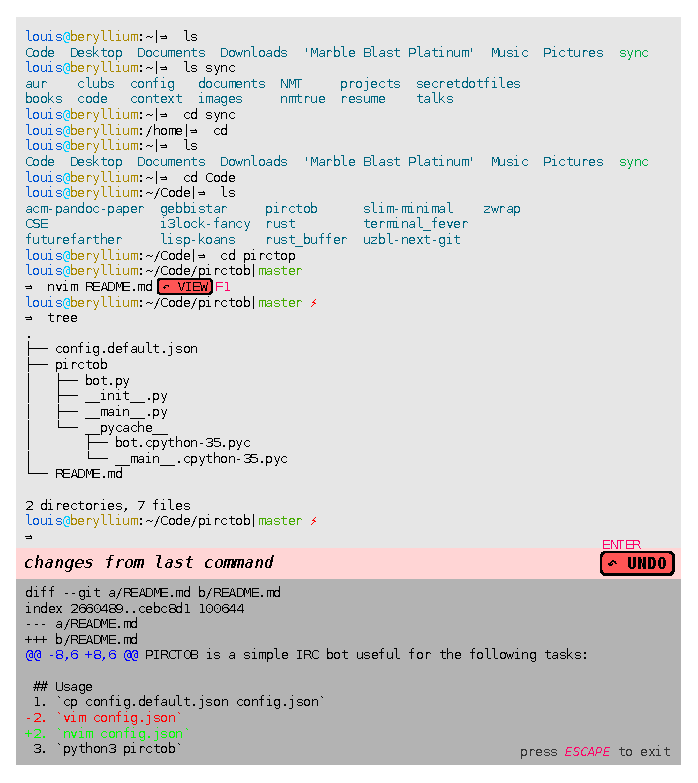
\includegraphics[width=0.8\linewidth]{figures/interface/undo.eps}
  \caption{A mockup of the undo window with undo option}
  \label{fig:undo}
\end{figure}

In Figure \ref{fig:undo} we can see an example interface for the undo window for
our terminal. After a command is entered that changes something, this shows the
user exactly what changes have taken place, and makes it possible to undo the
last set of changes. After any state-altering command is entered at the CLI, a
button is appended to the command in the log which brings up the shown
dialog. The same dialog can be made available from the heads-up display in the
bottom, or the terminal can be configured to show the undo window after
destructive commands by default.

The point of this interface is to create an escape hatch to allow the user to
return the entire system to the state before the previous command. This is an
example of responsive disclosure, because the information is only made available
to the user when they indicate that they want to know how to undo a command. The
system is also inherently limited in that it can only undo a single command, so
as more commands are entered the button should disappear from older commands that can no longer be undone. This follows the principle of responsive enabling.

The undo button closes the pane by undoing the command, and pressing
\texttt{ESC} simply returns the user to the normal context window without
undoing anything. Both are examples of having a prominent ``done'' button, so
the user knows how to tell the terminal they're done with the undo dialog.


\section{Evaluation Planning}
\label{sec:eval}
Evaluating the effectiveness of our design is an important step in understanding
how we can and have effected users abilities with and knowledge of the command
line. An important metric for this would be \emph{unique command count} --- the
measure of how many unique commands the user is able to use. This includes
things such as looping, options, as well as actual commands. Our goal is to
understand the impact our designs could have on unique command count, as well as
general user experience.

We hypothesize the following:
\begin{itemize}
  \item Users who use our program will have a higher unique command count than
  the control group.
  \item Users who use our program will report a more positive user experience.
  \item Users who use our program will maintain their unique command count
  outside of our shell.
\end{itemize}
These captor the idea that the users should begin using the shell better, have
less fear of the shell, and will be able to carry this knowledge to other systems.

\subsection{Collecting Data}
Collecting data to this end will take place in two parts:
\begin{itemize}
  \item A user survey to gauge users emotional experience --- how much they
  enjoyed using the command line.
  \item A data reporting study, which would report command history for a number
  of users.
\end{itemize}
These would each need to be run for our two groups: control and enhanced. Likely
our study would require each group (of mixed experience levels), to use our
software for a period of time. Then we would give them a number of tasks to
perform. After they have completed the tasks, we can collect statistics, and
conduct the survey.

Our user survey would need to focus in on the emotional experience of our
users. It would ask questions such as
\begin{quote}
  \begin{itemize}
    \item Rank your intimidation of the system.
    \item Rank how hard it was to perform a given task.
    \item Rank how well you think you used the system.
    \item Rank how happy you were with your experience.
  \end{itemize}
\end{quote}

Automated usage statistics would be much easier. All we would need to do is get
the history file for each user, and look at the unique command usage.

Together we can use these to test the first two of our hypotheses. For the
third, we would require users to switch from our system to a traditional system
after an extended period. At that point we could likely re-conduct our analysis
to see if users have learned skills in a way they can reproduce.
\begin{figure}[ht]
  \centering
  \includegraphics[width=0.8\linewidth]{figures/user_study.png}
  \caption{\label{fig:ustud} This shows a timeline of how we would evaluate our
    design.}
\end{figure}
Figure \ref{fig:ustud} shows something of a timeline on how this would work to
develop our understanding. Again, in it we have two groups of users. Each
receives training in a different command line system. Each will be given a set
of tasks after some period of time. After these tasks, we can begin to analyze
the results.



%%% Local Variables:
%%% mode: latex
%%% TeX-master: "documentation"
%%% End:


\section{Results}
\label{sec:results}
Data for our preliminary results were collected using Google Forms. The
prototype would issue information to the user to take an entry survey, guide
them through the features, and finish with an exit survey. The two surveys
contained the following questions:

\begin{center}
  \begin{tabular}{|l|p{0.6\linewidth}|}
    \hline
    \multicolumn{2}{|c|}{\Large \textbf{Entry Survey}}\\
    \hline
    \multirow{6}{*}{\textbf{Demographics}}
 & Name \\ \cline{2-2}
 & Age \\\cline{2-2}
 & Gender \\\cline{2-2}
 & Education \\\cline{2-2}
 & Major \\\cline{2-2}
 & Primary OS \\
    \hline
    \multirow{6}{*}{\textbf{Usability of Shell}}
 & I think the command line is easy to use. \\ \cline{2-2}
 & I think the command line is more usable than a GUI. \\ \cline{2-2}
 & I feel comfortable using the shell. \\ \cline{2-2}
 & I prefer command line tools to GUI tools.\\ \cline{2-2}
 & I think I would prefer the shell if I understood it better (or already
   do).\\ \cline{2-2}
 & I think the shell is easy to learn.\\
    \hline
    \multirow{4}{*}{\textbf{Efficiency}}
 & I use piping and redirection. \\ \cline{2-2}
 & I use control structures in the shell.\\ \cline{2-2}
 & I use wild cards in the shell.\\
    \hline
    \multirow{5}{*}{\textbf{Knowledge}}
 & When presented with a problem, I know the commands to use. \\ \cline{2-2}
 & I feel that learning how to use new commands is easy. \\ \cline{2-2}
 & I use a wide array of commands. \\ \cline{2-2}
 & I feel that I have sufficient knowledge of the shell for what I need. \\
    \hline
    \multirow{1}{*}{\textbf{Qualitative}} & Explain what tasks you commonly carry
                                            out on in the shell.\\
    \hline
  \end{tabular}
\end{center}

\begin{center}
  \begin{tabular}{|l|p{0.6\linewidth}|}
    \hline \multicolumn{2}{|c|}{\textbf{\Large Exit Survey}} \\ \hline
    \multirow{4}{*}{\textbf{Usability}}
    & This system would improve my usage of the shell. \\ \cline{2-2}
    & This system would help me solve problems in the shell. \\ \cline{2-2}
    & This system is more usable than a traditional shell. \\ \cline{2-2}
    & I find the interface of the system inviting and usable. \\
    \hline
    \multirow{3}{*}{\textbf{Educational Value}}
    & This system would teach me commands in a more effective way than the
      status quo. \\ \cline{2-2}
    & This system would help me perform automation that I would not make on my
      own.\\ \cline{2-2}
    & Using this system would improve my understanding of all shells.\\
    \hline
    \multirow{3}{*}{\textbf{Intention}}
    & I would prefer this to the normal shell experience. \\ \cline{2-2}
    & I would use this system in the future. \\ \cline{2-2}
    & I would suggest this system to others. \\
    \hline
    \multirow{2}{*}{\textbf{Qualitative Critique}}
    & What did you like most about the system?  \\ \cline{2-2}
    & What do you think needs the most improvements? \\
    \hline
  \end{tabular}
\end{center}
In between these surveys we presented a demo of our system.

\subsection{Data Analysis}
Data analysis was carried out using the Julia and Python languages, along with
various statistical tools. A cursory data analysis was also provided by Google
Sheets, allowing an overview of the results from each question.

The first thing we want to do is understand the demographics of our
survey. Primarily, and somewhat unsurprisingly, the primary responding group was
male CS majors. Linux was the dominant operating system, but not exclusive. The
reported education levels were diverse, spanning from the sophomore to graduate
levels.

% TODO: Probably make subfigs for this data?
\begin{figure}[ht]
  \centering
  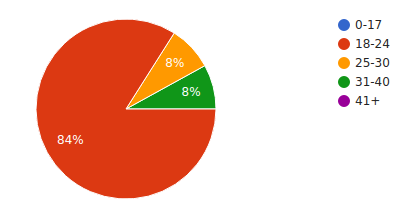
\includegraphics[width=0.8\linewidth]{figures/stats/age.png}
  \caption{\label{fig:age} Age demographics of survey base. }
\end{figure}

\begin{figure}[ht]
  \centering
  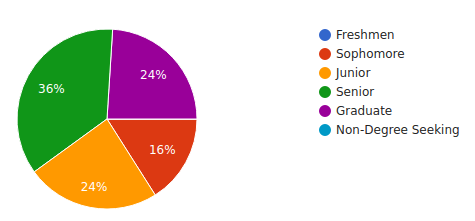
\includegraphics[width=0.8\linewidth]{figures/stats/edu.png}
  \caption{\label{fig:edu} Education demographics of survey base. }
\end{figure}

\begin{figure}[ht]
  \centering
  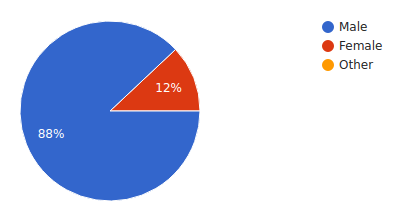
\includegraphics[width=0.8\linewidth]{figures/stats/gender.png}
  \caption{\label{fig:gender} Gender demographics of survey base. }
\end{figure}

\begin{figure}[ht]
  \centering
  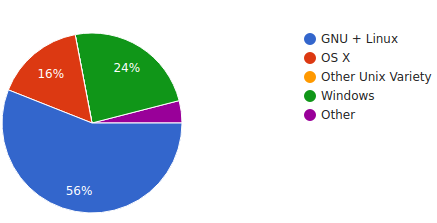
\includegraphics[width=0.8\linewidth]{figures/stats/os.png}
  \caption{\label{fig:OS} OS demographics of survey base. }
\end{figure}

We used the following Julia code to analyze the relative skill levels of our
users. Simply summing up the comfort level of all questions on the Entry survey,
we ranked users from Novice (0 experience) to Expert (39). Figure
\ref{fig:skill} shows a histogram representing user skill. You will notice that
the majority of our users are more experienced (self-reportedly). This does not
align with our target audience, however there was novice representation.
\begin{figure}[ht]
  \centering
  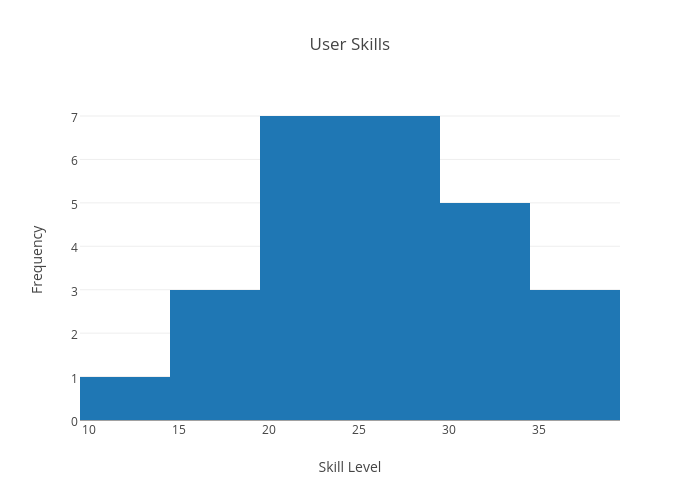
\includegraphics[width=0.8\linewidth]{figures/stats/user-skills.png}
  \caption{\label{fig:Skill} Histogram showing the relative skill levels of the
    user base. Note the larger right tail. }
\end{figure}

To get a better understanding of how our users were grouped we conducted several
standard pearson product-moment correlation coefficient analysis'. Firstly, we
compared how users were most significantly grouped by how they answered the
entry and exit surveys. Figure \ref{fig:p_plot} shows these results in a
graphical form, with the table available in Appendix \ref{fig:p_table}. Marked
in color are the correlation values in all instances where the p-value is
significant (less than 0.05). A divergent colormap is used: red indicating
negative correlation, the darker the stronger; blue indicating positive
correlation, the darker the stronger. Everything less than significant has been
omitted for clarity.

From the entry survey the most widely associable response is a user's answer to
the question "I feel comfortable using the shell". This responses to this
question have a positive correlation to two responses under the efficiency
vector, three responses under the knowledge vector, a single question under the
usability vector, and two questions under the education vector. This shows that
users who are more comfortable with using the shell are also more likely to be
skilled users of it, unsurprisingly. From the exit survey questions, this graph
shows that users who self-reported being more comfortable with the shell also
found the prototype more usable.

From the exit survey the most widely associable response is a user's answer to
the question "The system would improve my usage of the shell." The responses to
this question are positively correlateable to every other question on the exit
survey.

The only significant negative correlation is between two question on the entry
survey: "I use control structures in the shell" and "I think I would prefer the
shell if I understood it".

\subsection{Qualitative Analysis}
    8d. Describe the quantitative/qualitative analysis results with proper
    statistics test/grounded theory. You should also indicate whether or not the
    analysis result can support the hypotheses in Section 8.

Our entry and exit surveys each had at least one qualitative response question.
The responses to these can be seen in Appendix \ref{fig:fig_data}.
The entry survey asked users what tasks they commonly carried out in the shell.
Seven out of the fifteen responses indicated navigation and file manipulation,
five indicated programming-related tasks, and four indicated searching.

There were two qualitative response questions on the exit survey. The first
asked users what they liked most about the prototype. There is no clear
consensus here - users reported liking the GUI elements, the context window, the
undo functionality, the suggested automations, and other disparate features.

The second asked users what they thought needed the most improvement in the
prototype. Three users indicated that more information is needed in the
interface; one wrote: "More instructions on what the buttons on bottom will do
if pressed would be nice-- I know the functionality of the buttons isn't
implemented yet, but a small message explaining what the buttons represent and
happens when they are clicked would go a long way". Two users reported confusion
with the prototype. Five did not provide an answer or indicated that they had no
suggestions.

%%% Local Variables:
%%% mode: latex
%%% TeX-master: "documentation"
%%% End:


\section{Conclusion}
\label{sec:conclusion}
Throughout this report, we have demonstrated a collection of enhancements that
could be made to the typical Unix command line shell in order to increase the
efficiency, usability, and understand-ability of the system. Targeting those
learning Unix for the first time, we hoped to demonstrate ways to help teach
beginners, by bringing common GUI techniques to the command line. Once we have
left the prototype phase, a more extensive analysis can be carried out, as
described in Section \ref{sec:eval}.

Thus far we have designed a basic web-based prototype of the system, one that
highlights it's novel GUI techniques and core functionality. As is discussed
above, we've gone through a preliminary user study of our prototype. This study
consisted of an entry survey to gauge users' prior experience with the shell,
and attitudes towards the shell. Following a walkthrough of the prototype, we
queried users on their experience: whether they found it usable, educational,
and enjoyable. These results can now be used to evaluate and refine the
prototype in response to users' critiques.

In Section \ref{sec:results} we analyzed the user responses to both surveys. This
section of testing was intended to test the hypothesis that users who use our
program would report a more positive user experience. On the entry survey
querying a user's self-reported experience with the shell with regards to
usability, efficiency, and knowledge users reported an average rating of 1.9,
2.2, and 2.0 respectively (from 1 to 4 in a Likert-style questionnaire). On the
exit survey users ranked the prototype a 1.9, 1.7, and 1.9 on its usability,
educational potential, and their experience with it respectively (from 1 to 4 in
a Likert-style questionnaire).

Based upon these ratings, we conclude that our hypothesis here is not supported
by the reactions to this prototype. The command line interface certainly can be
made more user friendly by the application of user interface design techniques,
and more work and research on our prototype can help us accomplish that goal in
the future.

% \emph{THE END}

% From the responses we can speculate a bit as to why, and how we can improve
% future versions of the application.

% * users did not find the design compelling
% * users found the interface confusing
% * users %...

% 9a. Briefly describe what the system is and how you evaluate the system
% 9b. Use a list to describe which hypotheses in Section 7 are supported in the evaluation
% 9c. (optional) List the findings which are in the hyphteses.
% 9d. (optional) List possible strategies to enhanced the system .
%%% Local Variables:
%%% mode: latex
%%% TeX-master: "documentation"
%%% End:


\bibliographystyle{acm}
\bibliography{bib}

\end{document}
%%% Local Variables:
%%% mode: latex
%%% TeX-master: t
%%% End:
